\documentclass{article}
\usepackage{amsmath}
\usepackage{listings}
\usepackage{moreverb}
\usepackage[margin=1in]{geometry}
\usepackage{graphicx}
\usepackage{dsfont}
\title{STA 360: Assignment 1}
\author{Michael Lin}

\begin{document}
\maketitle

\begin{enumerate}
\item The formula for the posterior density, $p(\theta|x_{1:n})$, is derived using Bayes' theorem and plugging in the likelihood and prior:
\begin{align*}
p(\theta|x_{1:n})&=p(x_{1:n}|\theta)p(\theta) \\
&=\prod\limits_{i=1}^{n}\theta \exp(-\theta x_i) \mathds{1}(x_i>0)\frac{b^a}{\Gamma(a)}\theta^{a-1}\exp(-b\theta)\mathds{1}(\theta>0) \\
&=\theta^n\exp(-\theta\sum\limits_{i=1}^{n}x_i) \mathds{1}(x_i>0)\frac{b^a}{\Gamma(a)}\theta^{a-1}\exp(-b\theta)\mathds{1}(\theta>0) \\
&\propto \theta^{a+n-1}\exp\{-\theta(b+\sum\limits_{i=1}^{n}x_i)\}\mathds{1}(\theta>0) \\
&\propto \mathrm{Gamma}(\theta|a+n, b+\sum\limits_{i=1}^{n}x_i)
\end{align*}
Thus, the posterior density is $$ \mathrm{Gamma}(\theta|a+n, b+\sum\limits_{i=1}^{n}x_i) $$

\item The prior density is Gamma(0.1,1.0). Using the formula derived from part 1, we have that the posterior density is Gamma(8.1,155.5). Their plots are displayed below.

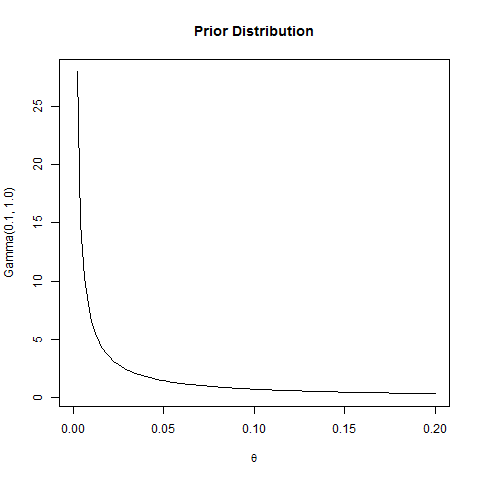
\includegraphics[scale=0.45]{prior}
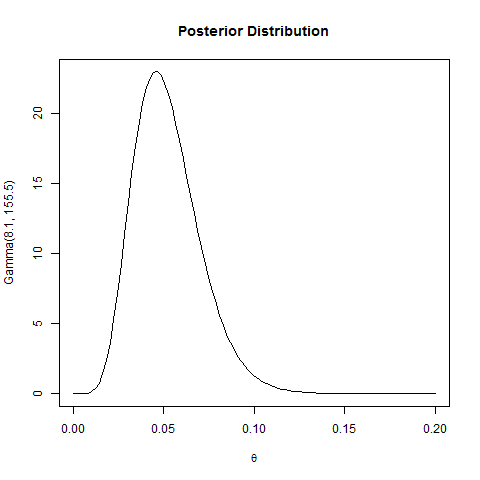
\includegraphics[scale=0.45]{post}

\pagebreak

See below for R code used to plot prior and posterior p.d.f.s.

\listinginput[1]{1}{assign1code.r}


\end{enumerate}
\end{document}